\documentclass[a4paper,12pt]{article}
\usepackage{fontspec}
\usepackage{polyglossia}
\setmainlanguage{russian}
\setotherlanguage{english}

\usepackage{amsmath}
\usepackage{amssymb}
\usepackage{geometry}
\usepackage{graphicx}
\usepackage{hyperref}
\usepackage{xcolor}
\usepackage{minted}
\usepackage{fvextra}
\usepackage{tikz}
\usepackage[normalem]{ulem}

\usemintedstyle{trac}

\geometry{top=2cm,bottom=2cm,left=2cm,right=2cm}

\setmainfont[Path = ../fonts/]{centuryschoolbook.ttf}
\newfontfamily\cyrillicfont[Path = ../fonts/]{centuryschoolbook.ttf}
\newfontfamily\cyrillicfontsf[Path = ../fonts/]{centuryschoolbook.ttf}
\newfontfamily\cyrillicfonttt[
	Path = ../fonts/,
	UprightFont = *-Regular.ttf,
	ItalicFont = *-Italic.ttf,
	BoldFont = *-Bold.ttf,
	BoldItalicFont = *-BoldItalic.ttf
]{AdwaitaMono}

\setmonofont[
	Path = ../fonts/,
	UprightFont = *-Regular.ttf,
	ItalicFont = *-Italic.ttf,
	BoldFont = *-Bold.ttf,
	BoldItalicFont = *-BoldItalic.ttf
]{AdwaitaMono}

\title{Алгоритмы и структуры данных. Линейные алгоритмы}
\author{densine}
\date{\today}

\begin{document}

\maketitle
\tableofcontents

\section{Префиксы/суффиксы}

\subsection{Определение}

Пусть у нас есть массив из $n$ чисел - например $[a_1, a_2 \dots a_n]$, а также
$q$ запросов $[l, r]$. Для каждого запроса вывести:
\[
	a_l + a_{l+1} + \dots + a_r
\]

Как нам эффективно считать такую сумму?

\begin{itemize}
	\item Если мы будем пересчитывать ее каждый раз, то выйдет сложность $O(n * q)$.
	      Скажем, слишком долго.
	\item Введем понятие \uline{префикс массива} - отрезок от 0 до текущего элемента массива
	      \textendash\ $a_1, a_2 \dots a_r$. Суффикс \textendash\ аналогино от n до текущего элемента.
	      Что мы можем делать с этим префиксом? Посчитать его сумму.
	      Из его определения следует, что префиксная сумма для $k$ равна префиксной
	      сумме для $k - 1$ плюс $a_k$.
	      \begin{minted}[frame=single]{cpp}
vector<int> pref(n + 1);
// pref[i] - сумма на [0;i), т.е. i - длина префикса
for (int i = 0; i < n; ++i) {
    pref[i + 1] = pref[i] + a[i];
}
          \end{minted}
	      Пример: есть массив $x = [1, 6, 7, 3, 5, 8]$.
	      Тогда $pref_x = [0, 1, 7, 14, 17, 22, 30]$.
\end{itemize}

Затем, с помощью префиксных сумм можно очень быстро находить суммы любых
сплошных отрезков в массиве! Нужно просто вычесть из одной суммы другую
- т.е. из отрезка длины $r$ отрезок длины $l$. Тогда из суммы первых
$r$ элементов мы вычтем сумму первых $l$ элементов. Логично, что
останется сумма элементов $(l, r]$.

\subsection{Код}

Выглядит это как-то так:

\begin{center}
	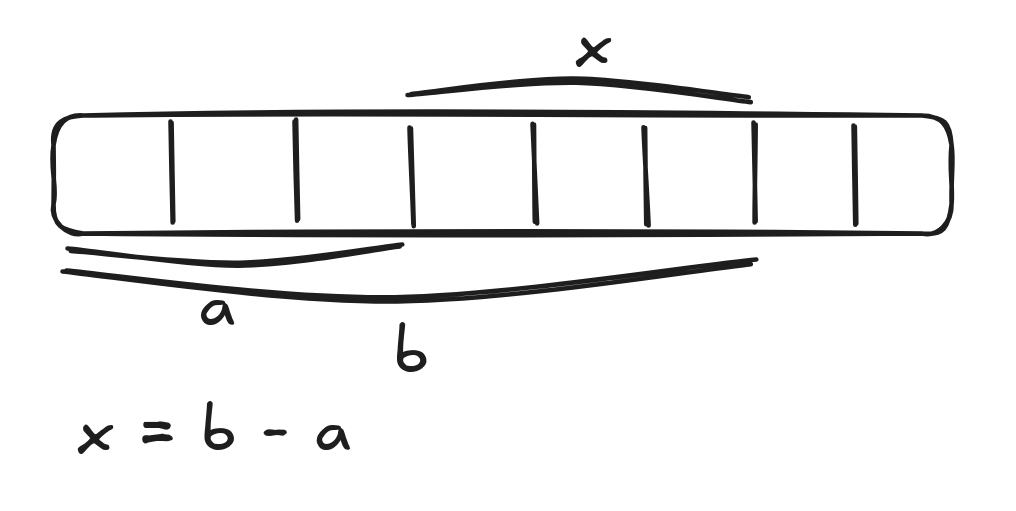
\includegraphics[width=0.7\textwidth]{../assets/prefsums.png}
\end{center}

Или с помощью кода:

\begin{minted}[frame=single]{cpp}
for (int i = 0; i < q; ++i) {
    int l, r;
    std::cin >> l >> r;
    l--;
    std::cout << pref[r] - pref[l] << std::endl; // '\n'
}
\end{minted}

Дальше шло 5-10 минут распинания о том, что использование символа
новой строки лучше чем $std::endl$.
По-моему же, если ваш код не справляется со временем, то никакое
отсутсвие $std::endl$ вам не поможет :).

Если вы вдруг задумали использовать этот алгоритм в задаче, в которой меняется
массив - имейте ввиду, что по идее после каждой операции все нужно будет
пересчитывать.

Префиксы можно использовать и для хранения произведения. Также для максимумов,
но тогда их и использовать как максимумы префиксов.

Итак, сложность такого алгоритма выходит $O(n + q)$.

\subsection{Примеры}
\begin{itemize}
	\item Дан массив $a_1, a_2 \dots a_n$. Найти максимальную сумму
	      подотрезка $(l,r)$.
	      \begin{minted}{cpp}
pref[r] - pref[l] // Это значение должно быть максимальным;
          \end{minted}
	      r перебираем. Берем l <= n такое, что pref[l] - min.
	      Полный код:
	      \begin{minted}[frame=single]{cpp}
int ans = 0;
int min_pref = 0;
for (int i = 0; i < n; ++i) {
    min_pref = std::min(min_pref, pref[i + 1]);
    if (pref[i + 1] - min_pref > ans) {
        ans = pref[i + 1];
    }
}
          \end{minted}
\end{itemize}

\subsection{Двумерные префиксные суммы}
Пусть нам дана матрица $n$ x $m$. Запросы имеют вид $x$ $y$ $u$ $v$.
Необходимо найти сумму элементов в подматрице от $(x,y)$ до $(u,v)$. Для
удобства иллюстрации площадью будем называть сумму всех чисел в подматрице
от $(x, y)$ до $(u, v)$.
\begin{center}
	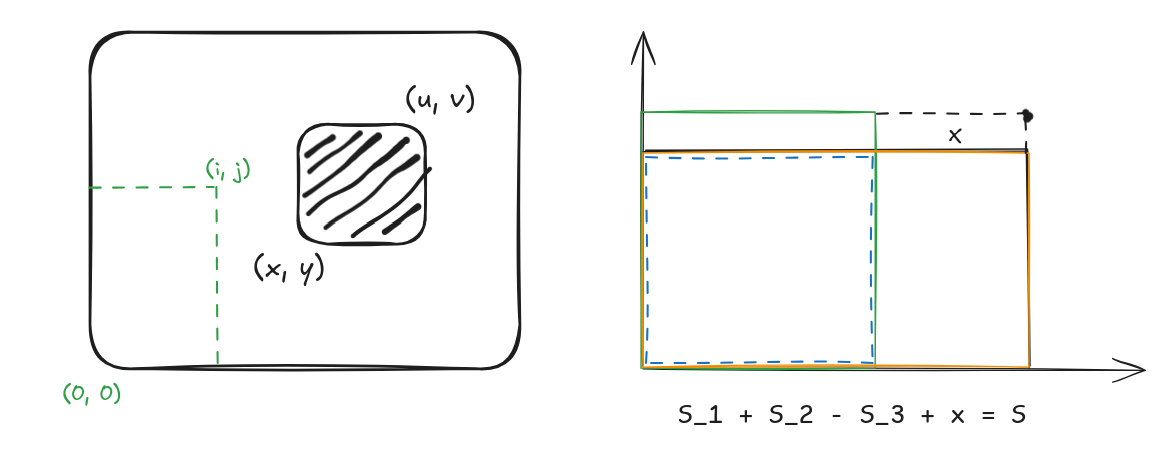
\includegraphics[width=0.95\textwidth]{../assets/matrixprefsum.png}
\end{center}

Для клетки ($i$,$j$) считаем сумму как:
\begin{minted}[frame=single]{cpp}
pref[i][j] = x[i][j] +
    pref[i - 1][j] + pref[i][j - 1] - pref[i - 1][j - 1];
\end{minted}
где $x[i][j]$ соотвествует сумме белого прямоугольника, $pref[i - 1][j]$
площади зеленого, $pref[i][j - 1]$ \textendash\ оранжевого,
а $pref[i - 1][j - 1]$ \textendash\ остатка.
Иллюстрация на примере:
\begin{center}
	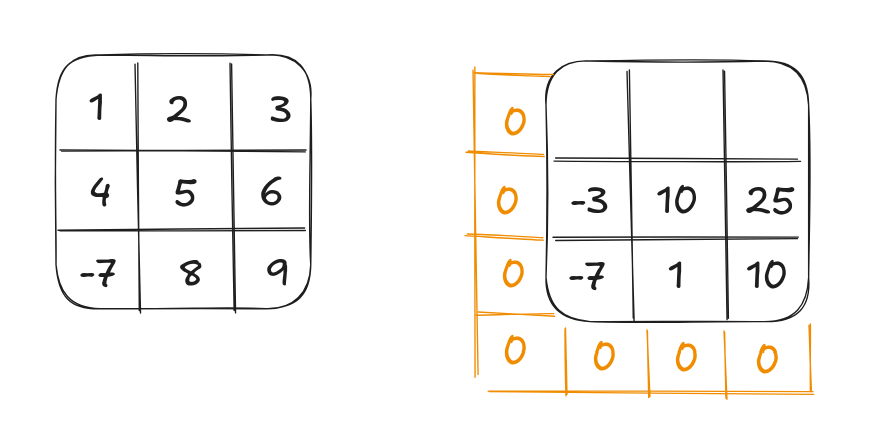
\includegraphics[width=0.7\textwidth]{../assets/mprefsumill.png}
\end{center}

Аналогично можно посчитать сумму не только следущей клетки в матрице
префиксных сумм, но и сумму подматрицы в данном двумерном массиве!
Снизу, аналогично, площадь фиолетового прямоугольника \textendash\
искомая. Пусть его левый нижний угол имеет координаты $(lx,ly)$, а
правый верхний \testendash\ $(rx,ry)$:

\begin{center}
	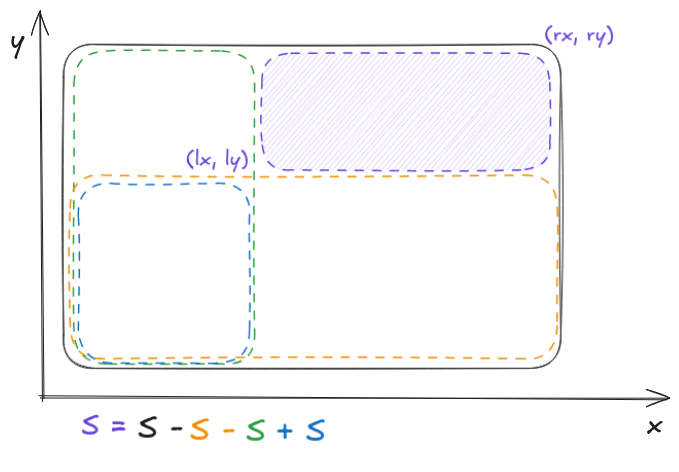
\includegraphics[width=0.7\textwidth]{../assets/submatrixsum.png}
\end{center}

Тогда площадью фиолотового треугольника является: \begin{minted}[frame=single]{cpp}
prefs[rx][ry]
    - prefs[rx][ly - 1] - prefs[lx - 1][ry]
    + prefs[lx - 1][ly - 1]
\end{minted}

\subsection{Алгоритм, поддерживающий изменения}
Пусть у нас есть массив $[a_1, a_2 \dots a_n]$, $q$ запросов вида
"прибавить $d$ к каждому числу $[a_l \dots a_r]$".
Будем хранить массив разностей!
\[
	x = [1, 5, 3, 8, 10];
	diffs_x = [1, 4, -2, 5, 2]
\]
В $diffs_x$ на первую позицию записываем $x_1$.
Далее $diffs_{x_i} = a_i - a_{i-1}$.
Тогда $x$ становится массивом префиксных сумм для $diffs_x$.
Затем, если мы хотим увеличить какие-либо $l - r + 1$ чисел,
то просто добавляем к $l$-ому элементу $diffs_x$ число $d$, а из
$r$-ого элемента $diffs_x$ число $d$ вычитаем:
\begin{center}
	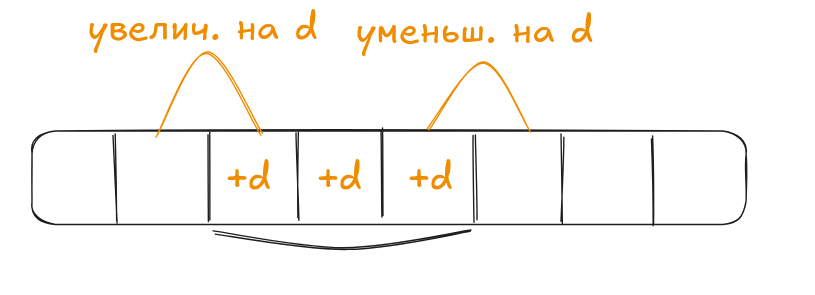
\includegraphics[width=0.7\textwidth]{../assets/diffarray.png}
\end{center}

Тогда код выглядит примерно так:

\begin{minted}[frame=single]{cpp}
std::vector<int> diff(n);
diff[0] = a[0];

// Заполняем массив разностей
for (int i = 1; i < n; ++i) {
    diff[i] = a[i] - a[i - 1];
}

// Обрабатываем каждый из запросов
for (int i = 0; i < q; ++i) {
    std::cin >> l >> r >> d;
    l--;
    diff[l] += d;
    diff[r] -= d;
}
\end{minted}

\subsection{Трехмерные префиксные суммы}
Реализация аналогична двумерному пространству \textendash\ советую насчет
данной преблемы найти информация в интернете. Замечу лишь что поиск подсуммы
имеет общее с формулой включений и исключений для множеств.

\section{Два указателя}
Какого-то общего описания алгоритма нет \textendash\ подход рассмотрим
на задачах, т.е. конкретных проблемах.
\begin{itemize}
	\item Допустим, у нас есть два массива:
	      $a_1 < a_2 < \dots < a_n$ и
	      $b_1 < b_2 < \dots < b_m$.
	      Задача \textendash\ за $O(n + m)$ найти $(i, j) : a_i = b_j$.
	      Например, если $a = (2, 3, 5)$ а $b = (1, 2, 4, 5)$, то пары это
	      $(i,j) = (0, 1)$ и $(2, 3)$.
	      Для каждого $i$ и $j$:
	      \begin{enumerate}
		      \item Если $a_i = b_j$, то добавляем пару $(i, j)$ в ответ и
		            инкрементируем оба указателя.
		      \item Если $a_i \neq b_j$ и $a_i < b_j$, инкрементируем $i$.
		            Иначе (если $a_i > b_j$), $j$.
	      \end{enumerate}
	      \begin{minted}[frame=single]{cpp}
std::vector<int> res;
int i = 0, j = 0;

while (i < n && j < m) {
    if (a[i] == b[j]) {
        res.push_back(a[i]);
        i++;
        j++;
    } else if (a[i] > b[j]) {
        j++;
    } else {
        i++;
    }
}
       	  \end{minted}

	\item Даны два массива: $a_1 \leq a_2 \leq \dots \leq a_n $ и
	      $b_1 \leq b_2 \leq \dots \leq b_m$. Задача - слить в один массив
	      по порядку все числа.
	      Просто по очереди перебираем числа из обоих массивов, и добавляем
	      то, что меньше и инкрементируем соответствующий указатель. Затем,
	      как только итерация по одному из массивов закочилась, докладываем
	      оставшиеся в другом массиве элементы. Код выглядит примерно так:
	      \begin{minted}[frame=single]{cpp}
int i = 0; j = 0;
std::vector<int> ans;
while (i < n && j < m) {
    if (a[i] <= b[j]) ans.push_back(a[i++]);
    else ans.push_back(b[j++]);
}

while (i < n) ans.push_back(a[i++]);
while (j < m) ans.push_back(b[j++]);
          \end{minted}

	\item Пусть нам дана прямая чисел $x_1 < x_2 < \dots < x_n$.
	      $#(i, j) : |x_i - x_j| \leq K$, где $i \leq j$ за O(n).
	      Количество пар для $i$-ой точки \textendash\ количество чисел
	      на отрезке $[x_i;x_i + k]$, т.е. нам просто нужно перебрать
	      для каждого $x_i$ по несколько $x_j$, находящихся после $x_i$ и
	      которые меньше чем $k$, а затем просто перейти к следующему
	      $x$.
	      \begin{minted}[frame=single]{cpp}
int i = 0, j = 0;
int count = 0;

for (i = 0; i < n; i++) {
    while (j < n && x[j] - x[i] <= k) j++;
    count += j - i;
}
		\end{minted}
\end{itemize}

\end{document}
